%update: Jan 15 fixed grammar according to prof notes
%update: Jan 09-11 prof check
%update: Jan 08 rephrased
%update: Dec 02 figures inserted
%update: Nov 29 citation done, bug fixes
%update: Nov 25 draft

%\begin{savequote}[75mm] 
%I see the world, not as it is, but as I are, or, as I are conditioned to see it.
%\qauthor{Stephen R. Covey} 
%\end{savequote}

\chapter{Statistically Analyzed Photoresponse of CdS Nanowires by \emph{in situ} TEM}

\newthought {To get the missing information for future flexible optoelectronics based on nanoscale building blocks}, as I discussed in Chapter 5, light, force and electrical currents are all important factors to be included into an {\it in siu} probing experiment. 
I demonstrate herein that high resolution TEM coupled with light illumination of a specimen and its electrical/mechanical probing can be applied for the {\em in situ} study of initiated photocurrents in free-standing individual nanowires. 
The crystallography of numerous individual CdS nanowires is analyzed simultaneously with the photocurrent measurements. 
My research implies that elastically deformed wurtzite CdS nanowires show statistically unchanged values of photo-to-dark current (ON/OFF) ratios. 
It is discovered that the cut-off wavelength possesses red shifts of photocurrent spectrum after nanowire bending. 
It is caused by deformation-induced lattice strain or associated changes in the electronic band structure, which is additionally proved by selected area electron diffraction (SAED) analyses and density functional tight binding (DFTB) calculations. 
The stable ratios of ON/OFF ratios, as well as photocurrent spectroscopy shifts of deformed CdS nanowires are important clues for future flexible optoelectronics and photovoltaics.\\

\begin{figure}  [ht]
\centering
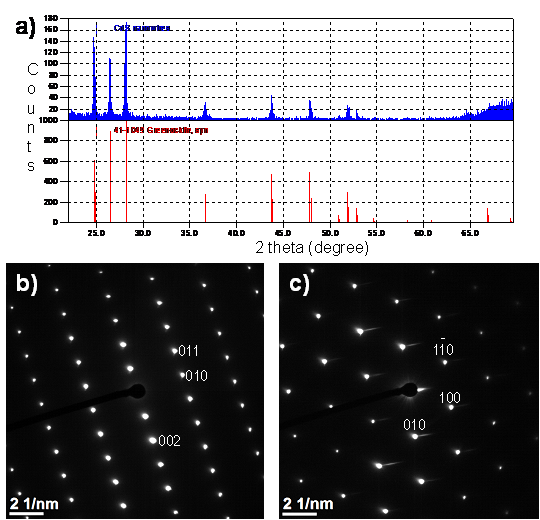
\includegraphics[width=0.8\textwidth]{figures/figure6_s1}
\caption[CdS crystallography]
{(a) XRD data of the nanowire sample (upper panel) fits a CdS hexagonal phase, JCPDS Card No. 41-1049 (lower panel). (b,c) Two SAED patterns of a CdS nanowire taken along the [100] and [001] directions, respectively. 
\label{fig:6_s1}}
\end{figure}

\section{Introduction}
As I mentioned in Chapter 1, flexible electronics and optoelectronics have attracted general public attentions in recent years because of the growing requirements for portable electronic devices having high performance and a low manufacturing cost.\cite{Boland2010,Liu2015,Long2012} 
With high surface-to-volume ratios, excellent carrier mobility and chemically decorated surfaces, which can further be modified/functionalized, one-dimensional inorganic semiconducting nanostructures are attractive candidates for lithium-ion batteries,\cite{Wang2015} future flexible displays,\cite{Klauk2008} solar cells,\cite{Zhang2012} supercapacitors,\cite{Li2014} nanogenerators,\cite{Fan2012} sensors,\cite{Zhang2014d} etc. \\
One of the crucial challenges for future applications is the nanostructure electrical and mechanical statistical stability. 
Although usually most reports claim that the nanowire conductivity is stable during mechanical deformations, there have been no deep and direct investigations related to the photoconductivity or photocurrent spectroscopy of free-standing individual nanowires under conditions which allow for the real-time observations of deformation-induced strains. \\
Hence, it is rather unclear how the crystallography changes in deformed nanowires affect their photoresponses. 
It is noteworthy that some materials were found to be unstable during elastic deformations.\cite{Antsov2014}
Herein, I thoroughly consider these issues by performing {\em in situ} HRTEM experiments using the optical TEM holder discussed in Chapter 2. \\

\begin{figure} [t] 
\centering
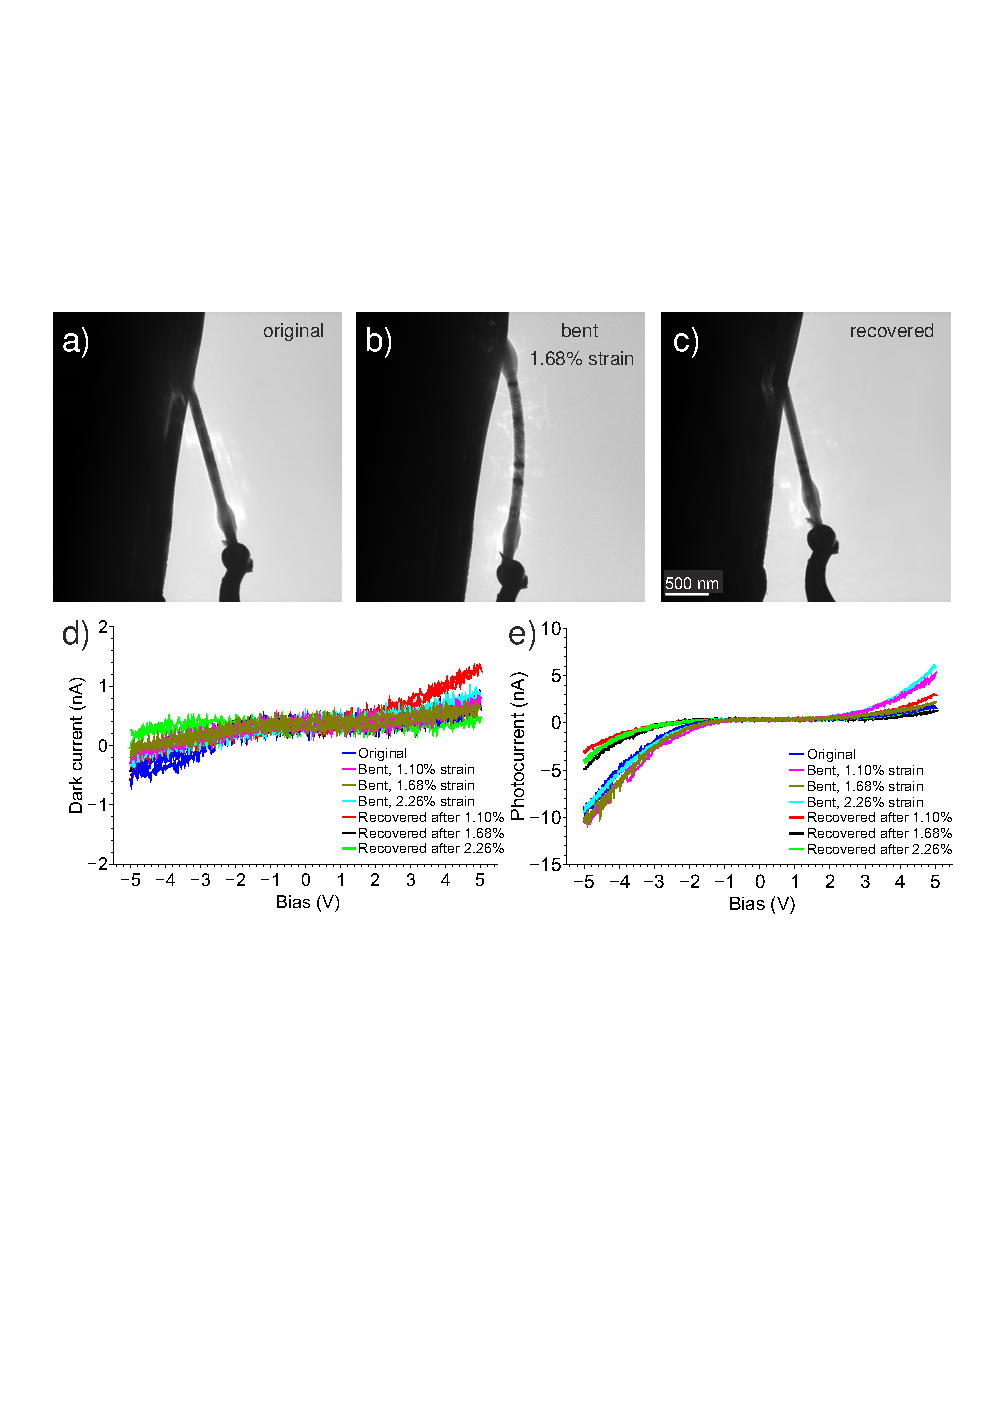
\includegraphics[width=\textwidth]{figures/figure6_2}
\caption[Deformation and I-V measurements]
{Representative TEM images of the original (a), bent (b) and recovered (c) states of an individual CdS nanowire positioned between fixed Au (left hand side) and movable W (right hand side) electrodes; and a summary of dark current (d) and photocurrent (e) measurements at different stages of the bending-recovery process. Calculated strains are marked on the TEM image and I-V plots. 
\label{fig:6_2}}
\end{figure}

I chose cadmium sulfide (CdS), a direct band gap semiconductor for diverse photoelectronic devices, as my testing nanowire material.\cite{Xing2015} 
Using paired probing and microscopy techniques, the electrical currents generated in light-illuminated specimen were measured by source-measuring units. \\
Initial testings revealed an unclear correlation between deformations and current values. 
To exclude the uncertainty introduced by the contact conditions, and to account for the structural diversity of the nanowires, I performed detailed statistical analysis based on numerous sets of experiments. 
Then the photocurrent spectroscopy measurements were performed. The spectroscopy reveals red-shifts for the cut-off wavelength of the nanowires under strain. 
The final part of the work attempts to characterize the strain-induced structural changes using electron diffraction analysis. 
\vfill

\section{Experimental}
CdS nanowires were synthesized via traditional chemical vapor deposition (CVD) method on silicon substrates or graphite plates. The fabrication conditions were reported in my published work.\cite{Zhang2015} 
The sizes of nanowires were around 100 nm in diameter and a few micrometers in length. 
The crystal structure of the nanowires was wurzite, which was confirmed by X-ray diffraction and SAED pattern, as shown in Figure \ref{fig:6_s1}. 
The samples were put onto a freshly-cut flattened gold wire tip by using a minimum amount of electrically-conductive silver epoxy. \\

As illustrated in Figure \ref{fig:6_1} in Chapter 2, the system is equipped with an optical fiber protruded through the TEM specimen holder, and with a piezo-tube for an electrical/mechanical probing inside the pole piece of the microscope. 
The probe with a tip radius ranging from 50 nm to several micrometers was aligned to the axis of the optical fiber core at a distance of ~0.5 mm. 
Probing, imaging and diffraction studies were conducted by using the same energy-filtered 300 kV JEM-3100FEF high-resolution TEM, under high vacuum ($10^{-5}$ Pa) at room temperature. 
For more information please refer to the description of engineering details of a piezo-driven optical TEM holder in Chapter 2.\\

\begin{figure}  [t]
\centering
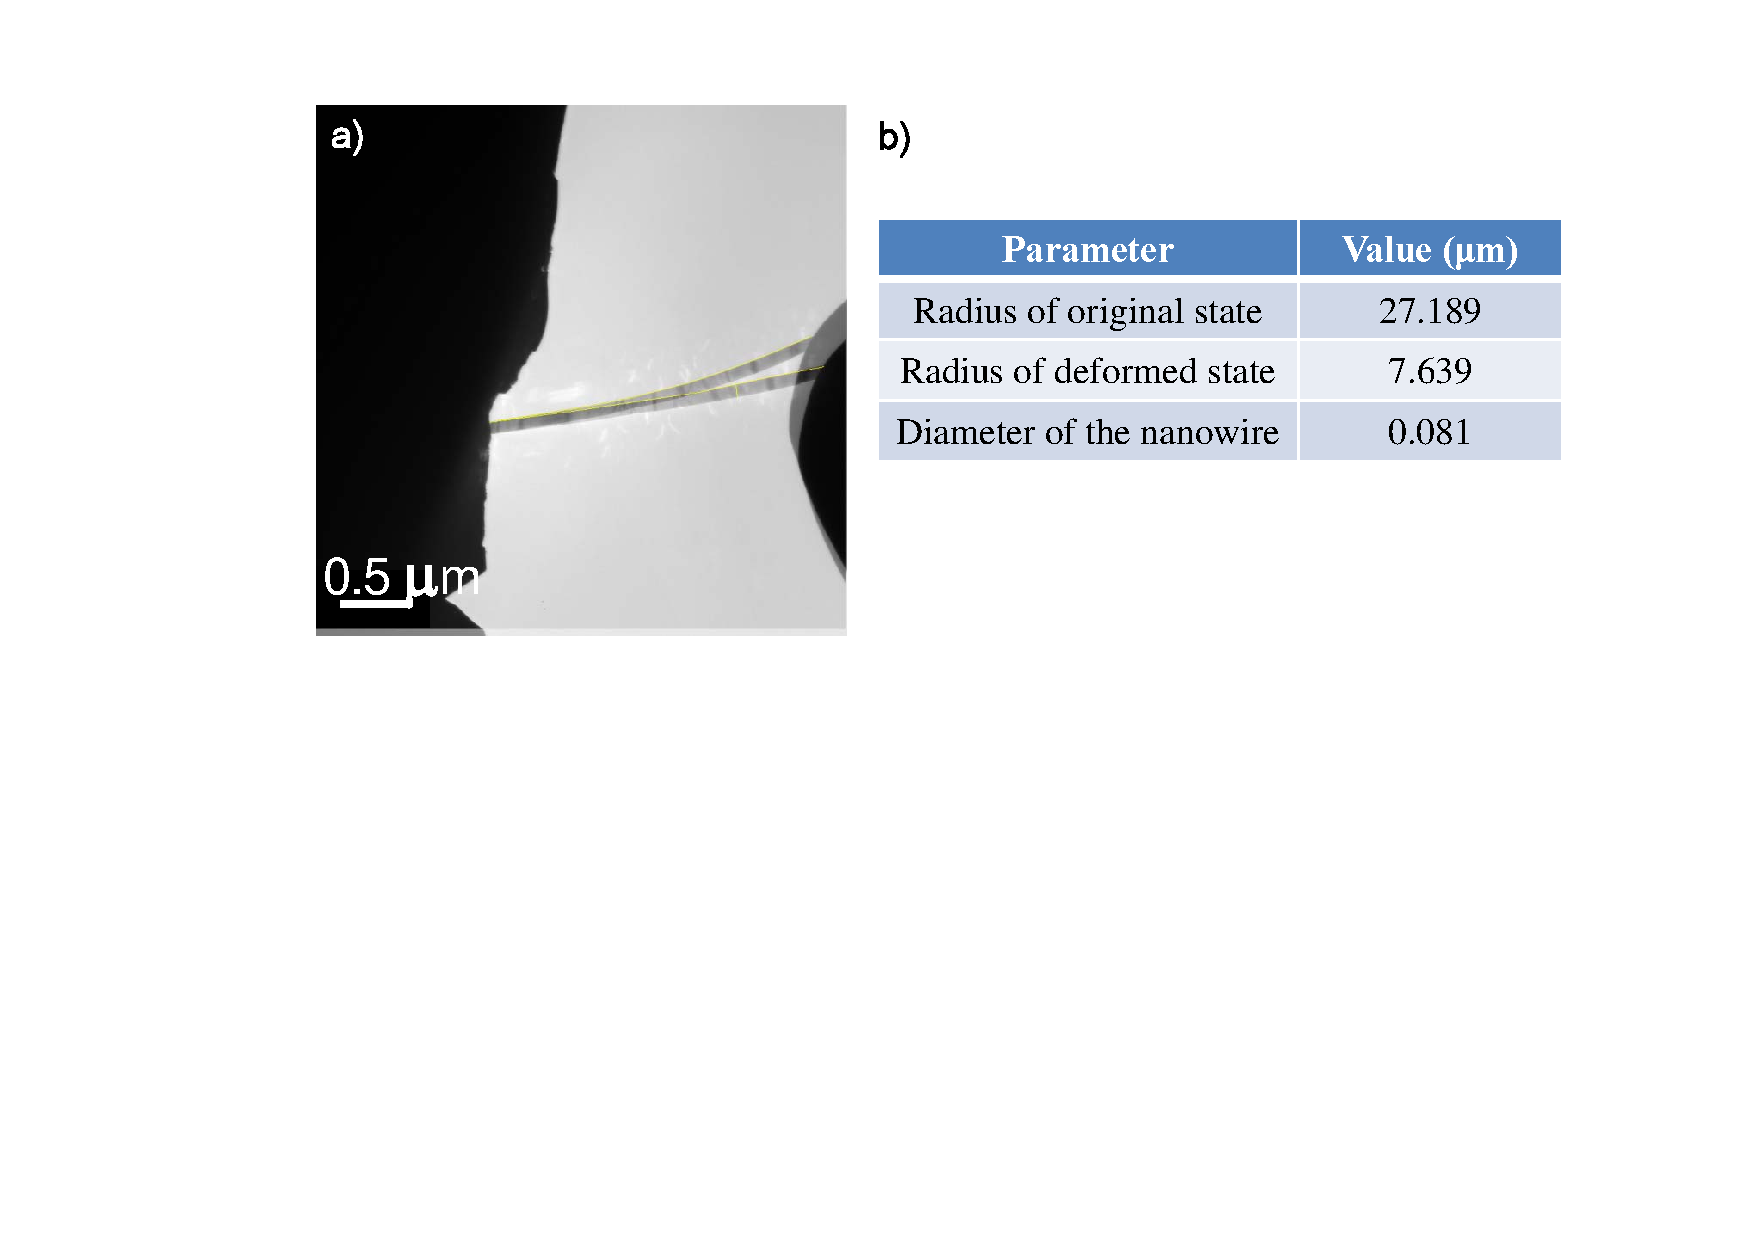
\includegraphics[height=\textwidth,angle=-90]{figures/figure6_s2}
\caption[Strain value]
{Strain values for an individual nanowire was determined under TEM imaging. 
(a) Two overlapped images of the nanowire in different states. 
(b) Measurements of the diameter of the nanowire, and its radius of curvature for the two cases. The strain was calculated as $d/R$, where $d$ and $R$ represent the diameter and the radius of curvature, respectively. The values were measured by using the {\em Digimizer} software\footnote{It is a free image analysis software from http://www.digimizer.com/}.
\label{fig:6_s2}}
\end{figure}

Two types of {\it in situ} experiments were conducted:\\
(1) Photocurrent I-V measurements, as illustrated in Figure \ref{fig:6_1} Scheme 1 in Chapter 2, while probing the I-V response of nanowires irradiated by a laser diode with a working wavelength of 488 nm. \\

(2) Photocurrent spectroscopy measurements, as described in Figure \ref{fig:6_1} Scheme 2 in Chapter 2, while measuring the wavelength dependency of the electrical current generated inside the nanowire under light illumination. 
The light source for photocurrent spectroscopy was a powerful laser driven light source (LDLS). The output of LDLS was then monochromated in order to carry out wavelength-selected measurements. 
In order to resolve the signal out of the noise, a chopper and a lock-in amplifier were applied in the measurement system. \\

\begin{figure}  [t]
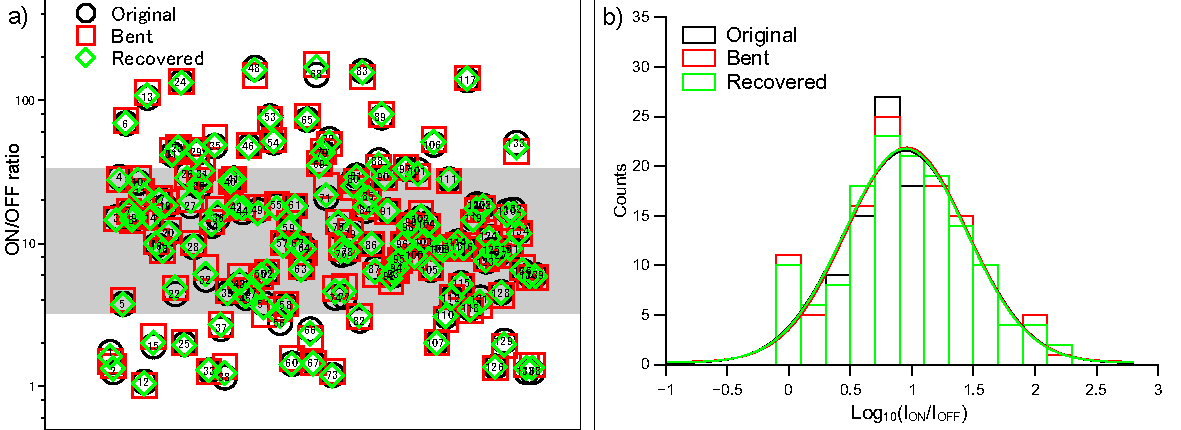
\includegraphics[width=\textwidth]{figures/figure6_3}
\caption[Statistical distribution of ON/OFF ratios]
{Statistical distribution of the measured ON/OFF (photocurrent/dark current) ratios for 139 bending/recovery experiments performed on free-standing single CdS nanowires. (a) ON/OFF ratios scatter mainly fits a gray region where the majority of measured ratios are included. (b) Statistical analysis of the ratios in log  scale. The lines represent Gaussian fits for the three histograms.
\label{fig:6_3}}
\end{figure}

\section{Results and discussions}
Photocurrents and dark currents of the nanowires were carefully measured by the sourcemeter before deformation, after it and after final and complete nanostructure recovery. 
Some of nanowires revealed stable contact properties during the deformations and recoveries, the other deviated from the stable behavior and possessed changed currents. 
Figure \ref{fig:6_2}a illustrates a contact to a nanowire in its original non-deformed state. \\

The average strain was defined as $\varepsilon = \frac{d}{R}$, where $d$ is the diameter of the nanowire, $R$ is its radius of  curvature.\footnote{Please not the the strain value determination here is the same as that in Chapter 5 in principle, but with a difference of constant factor of 2.} 
These two parameters were determined by a software, employing a curvature fit to the TEM images, as presented in Figure \ref{fig:6_s2} for a representative nanowire. 
I always try my best to get an intimate and stable physical contact, therefore the probe was slightly pressed towards the nanowire to avoid possible sliding between the probe and the specimen, as presented in Figure \ref{fig:6_2}a. 
The probe was then moved within the image plane for about 200 nm, leading to a strain of up to 1.68\%, as presented in Figure \ref{fig:6_2}b. 
The nanowire was finally recovered to its unbent state by moving the probe backwards, as illustrated in Figure \ref{fig:6_2}c. 
The I-V measurements were performed in both dark and illuminated conditions in each state, as summarized in Figure \ref{fig:6_2}d-e. 
In order to get a clear understanding of the correlation between the deformation states of the nanowires and the photocurrent responses, I performed numerous experiments for a comprehensive statistical analysis. 
The current values were found to be very much scattered. 
However, I found that the light ON/OFF ratio (photocurrent to dark current ratio) of the nanowires could be nearly stable. 

\begin{figure}[t]  
\centering
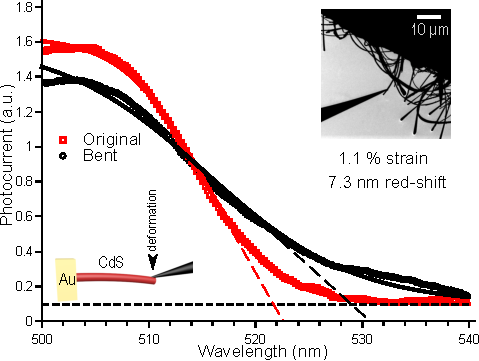
\includegraphics[width=250pt]{figures/figure6_4}
\caption[Photocurrent spectroscopy of deformed CdS NW]
{Photocurrent spectroscopy measurements performed on a representative individual CdS nanowire. The spectra have been fitted with logistic decay functions (solid lines); the regions of the curves corresponding to the symmetry point of each function have been extrapolated (dashed lines) to determine the intersections with the horizontal asymptote (dotted line). 
Left inset shows a schematic of the bending experiment. Right inset shows a low-magnification TEM image of the selected nanowire in contact with the W probe. 
\label{fig:6_4}}
\end{figure}

In this Chapter, I define three ON/OFF ratios, corresponding to the original, deformed and recovered states as:\\
{\center
$R_{ori} = \frac{I_{ph-ori}}{I_{dr-ori}}$, $R_{def} = \frac{I_{ph-def}}{I_{dk-def}}$, $R_{rec} = \frac{I_{ph-rec}}{I_{dk-rec}}$\\}

\vspace{5pt}, where $dk$ and $ph$ correspond to dark current and photocurrent, while $ori$, $def$ and $rec$ refer to the original, deformed and recovered states of the nanowire, respectively.\\

As presented in Figure \ref{fig:6_3}a, the values vary a lot for different cases. This might be caused by contact changes during probing, but the ON/OFF ratios are rather stable for each individual case. 
The statistical distributions of the ON/OFF values in Figure \ref{fig:6_3}b imply that this trend is valid in a wider scale and also allows us to estimate an average value of about 10, or around 7 to 20. 
The results of stable ON/OFF ratios made the majority of cases but some data had some deviations. 
Actually it is due to limitations of our setup with respect to the number of electrodes employed. These are only two. 
With only two electrical contacts, the contact resistance becomes an important uncertainty.\cite{Hummelgard2011} 
We expect that this variable could be reduced by the statistical analysis (on the basis that the contact resistance is normally randomly distributed). 
We expect that the nature of this variable (with respect to the resistance of the nanowire itself) allows for various contributions to be effectively separated. This enables us to observe the effects which are intrinsic to the nanowire samples themselves.

To get an additional information the photocurrent spectroscopy was performed under simultaneous TEM imaging. 

\begin{figure}  [t]
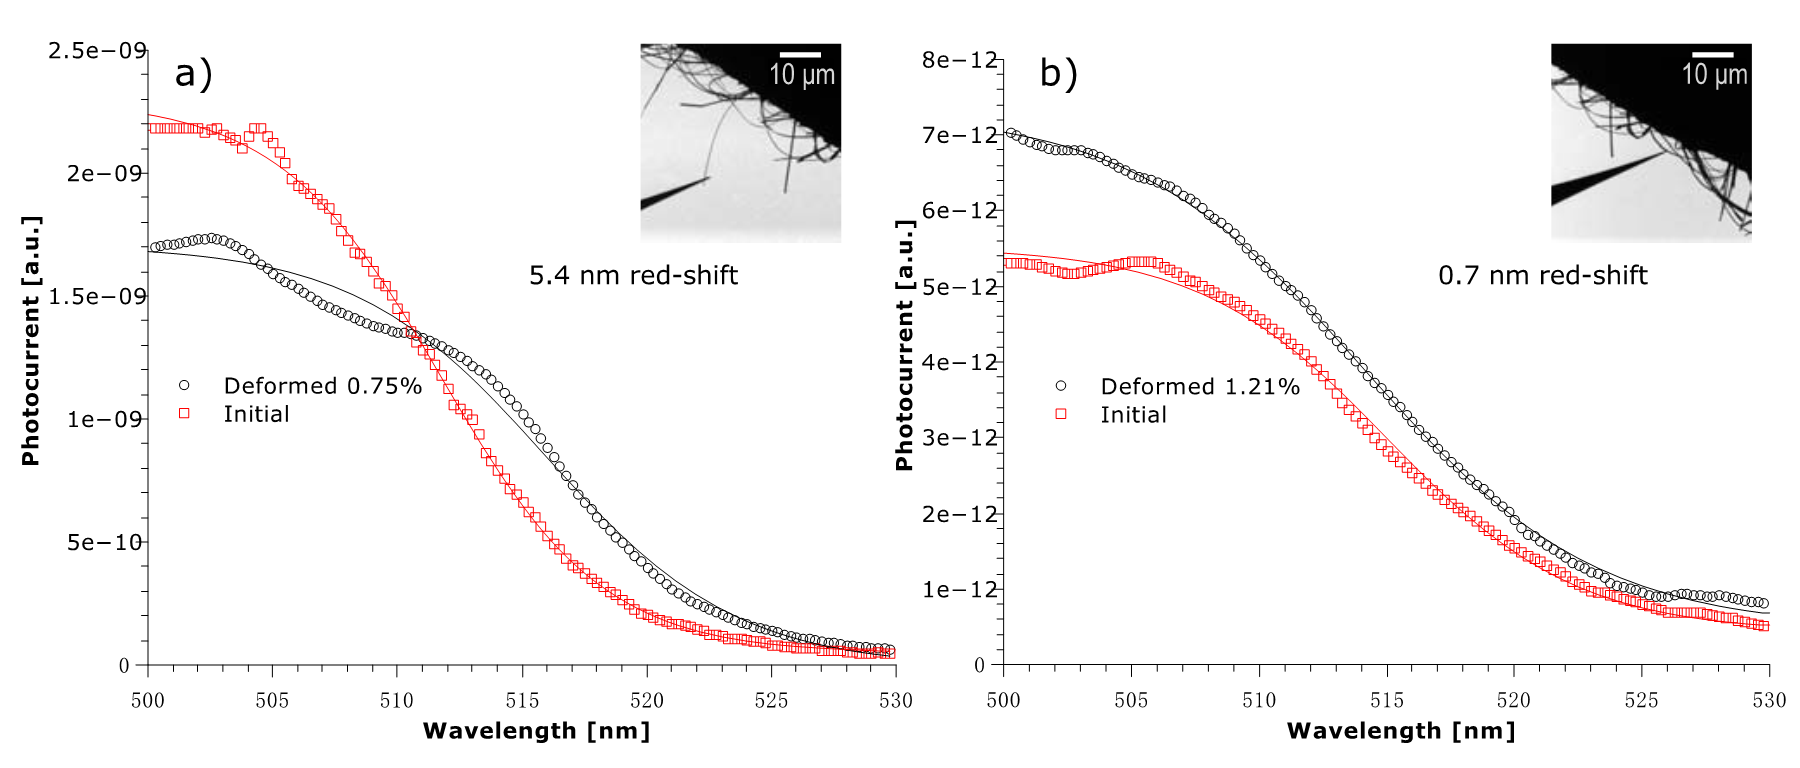
\includegraphics[width=\textwidth]{figures/figure6_s3}
\caption[Photocurrent spectroscopy of deformed CdS NW]
{(a,b) Additional examples of photocurrent spectroscopy on individual CdS nanowires, in their initial and deformed states. Low magnification TEM images are shown in the insets for each case. Strain and red-shift values are marked on each plot. 
\label{fig:6_s3}}
\end{figure}

In Figure \ref{fig:6_4}, the photocurrent spectroscopy results are plotted before and during the deformation process which introduces a 1.1\% elastic deformation.
The NW photocurrent cut-off wavelength possesses a 7.3 nm red shift under strain. At the initial state the edge wavelength was located at 521.8 nm. After deformation, the cut-off wavelength increased to 529.1 nm. 
More examples which feature similar red-shifts for the cut-off wavelength are shown in Figure \ref{fig:6_s3}. 
To sum up, the shifts of cut-off wavelength with regard to strains are listed in Table \ref{tab:6_1}. 

\begin{table}[b]
    \centering
    \begin{tabular}{c|c}
    \hline
         Strain (\%) & Red shifts (nm) (\%)\\
         \hline
         1.68 & 1.2\\
         0.75 & 5.4\\
         1.59 & -0.6\\
         1.21 & 0.7\\
         3.36 & 5.5\\
         \hline
    \end{tabular}
    \caption{Cut-off wavelength shift values for the independently deformed nanowires.}
    \label{tab:6_1}
\end{table}

Thus an average value of $3.3\pm2.9$ nm is obtained from Table \ref{tab:6_1}. The shift data shows that the effect is not limited to individual cases. 
The cut-off wavelength of the photocurrent spectrum is directly related to the electronic band structure. Thus it determines the near-band-edge emission (NBE) of the material. 
Our observations are consistent with the previous publications performed by measuring the CL of CdS nanowires inside SEM, where the authors observed red-shifted emission for the NBE peak under strain. 
This is an indication for a decrease in the bandgap value and it is in agreement with our data.\cite{Fu2011}

Evidence of the strain effects may cause the valence band decrease. Such strain effects may be observed by electron microscopy. 
Figure \ref{fig:6_5}ab presents the images of a CdS nanowire at the initial and deformed states. 
Insets of Figure \ref{fig:6_5}ab are SAED patterns from the area marked in Figure \ref{fig:6_5}ab. 

The averaged results presented here cannot accurately describe a single selected nanowire for its overall functional performance. 
In fact, the nanowires vary based on their morphology and structural peculiarities, even within the same synthetic batch of the material. 
There is a contradiction between the needs to accurately control the properties of every nanowire and the requirements for their high-yield production. However, from a statistical point of view, within a large number of structures, the nanowires studied here have common properties with respect to their photocurrent-to-dark current ratios. 


This means that the drawn conclusion is particularly important for devices fabricated by a large amount of nanowires (their bunches) instead of a single nanowire device. 
Some successful examples of making flexible photodetectors,\cite{Xu2015b} flexible transparent electrodes,\cite{Liu2014a} flexible supercapacitor electrodes,\cite{Liu2014a} LED arrays,\cite{Wang2015a} lithium-ion batteries,\cite{Wang2015} and solar cells,\cite{Zhang2012}, etc should be mentioned in this regard. \\

\begin{figure} [t] 
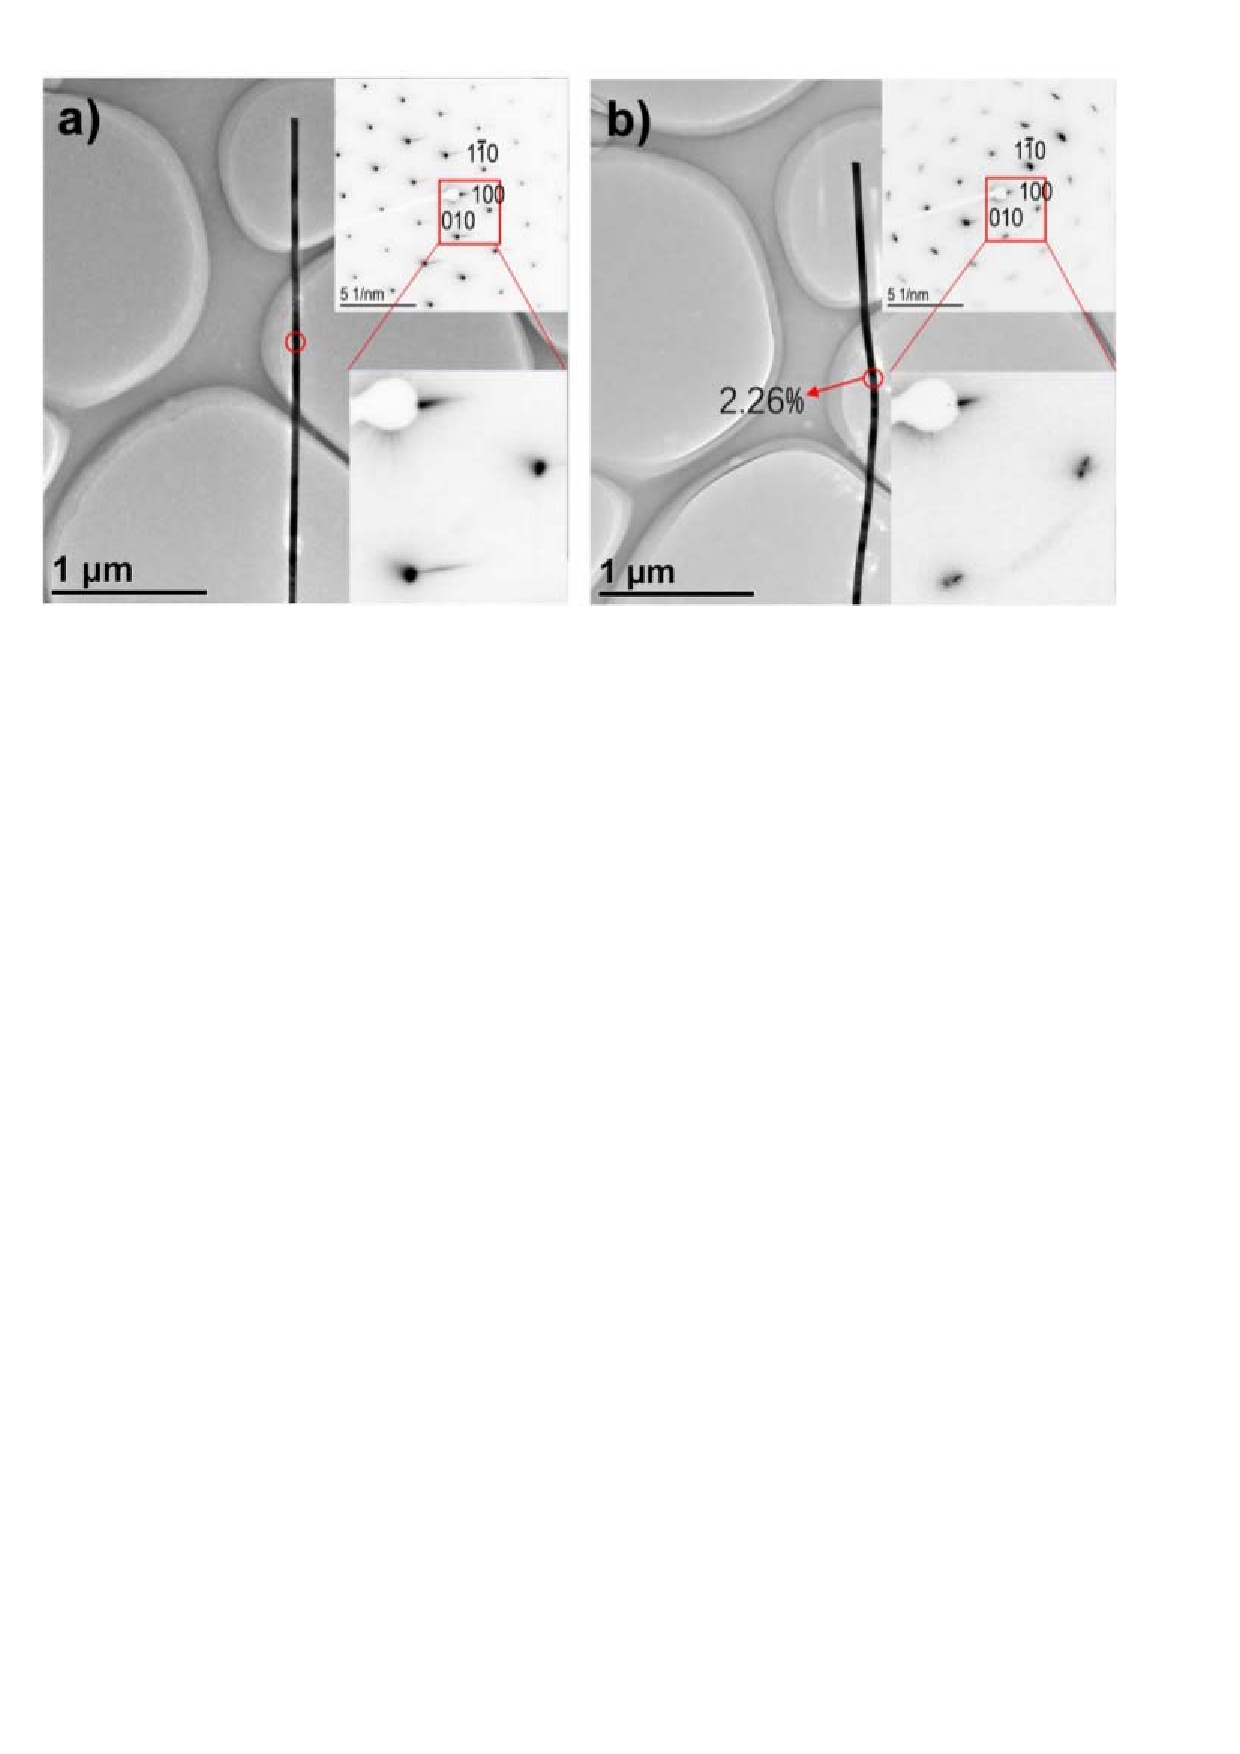
\includegraphics[width=\textwidth]{figures/figure6_5}
\caption[Diffraction of NW under strain]
{TEM images of the nanowire (a) before, and (b) after bending on a TEM carbon grid using a standard double-tilt holder due to the electron beam irradiation of the supporting C segments. 
The insets show SAED patterns along the [001] direction from areas marked by red circles. Representative framed parts of the SAED patterns are zoomed-in in the lower-right parts of the panels.
\label{fig:6_5}}
\end{figure}
\vfill


\section{Conclusions}
In conlusion, I have successfully performed photocurrent measurements for elastically deformed CdS nanowires inside the HRTEM. Using {\em in situ}  probing technique and the light illumination, I have characterized the electronic (dark current) and optoelectronic features of individual nanowires under mechanical deformation. 
To make the data reliable for future bottom-up applications, a large variety of nanowires was measured, which made possible an accurate statistical analysis of their properties. 
All nanostructures reveal fairly similar ON/OFF ratios in original, bent and recovered states, with this value mainly locating between 7 to 20. 
Photocurrent spectroscopy of several nanowires revealed red shifts of cut-off wavelength of several nanometers. 
These tiny shifts are mainly caused by deformation-induced strains, which induce changes in the electronic band structure. 
By taking SAED patterns, the strain induced structural deformation was vizualized after bending. 
The experiments reflect a variety of bending-induced stability features for individual nanowires. However, from a statistical point of view, the nanowires display common features in their response to deformation, making them highly valuable for future flexible optoelectronic applications. 

